\section{Referencia de la Clase List\-Almacen\-View}
\label{classListAlmacenView}\index{ListAlmacenView@{ListAlmacenView}}
Muestra y administra el listado de almacenes.  


{\tt \#include $<$listalmacenview.h$>$}

Diagrama de colaboraci\'{o}n para List\-Almacen\-View:\begin{figure}[H]
\begin{center}
\leavevmode
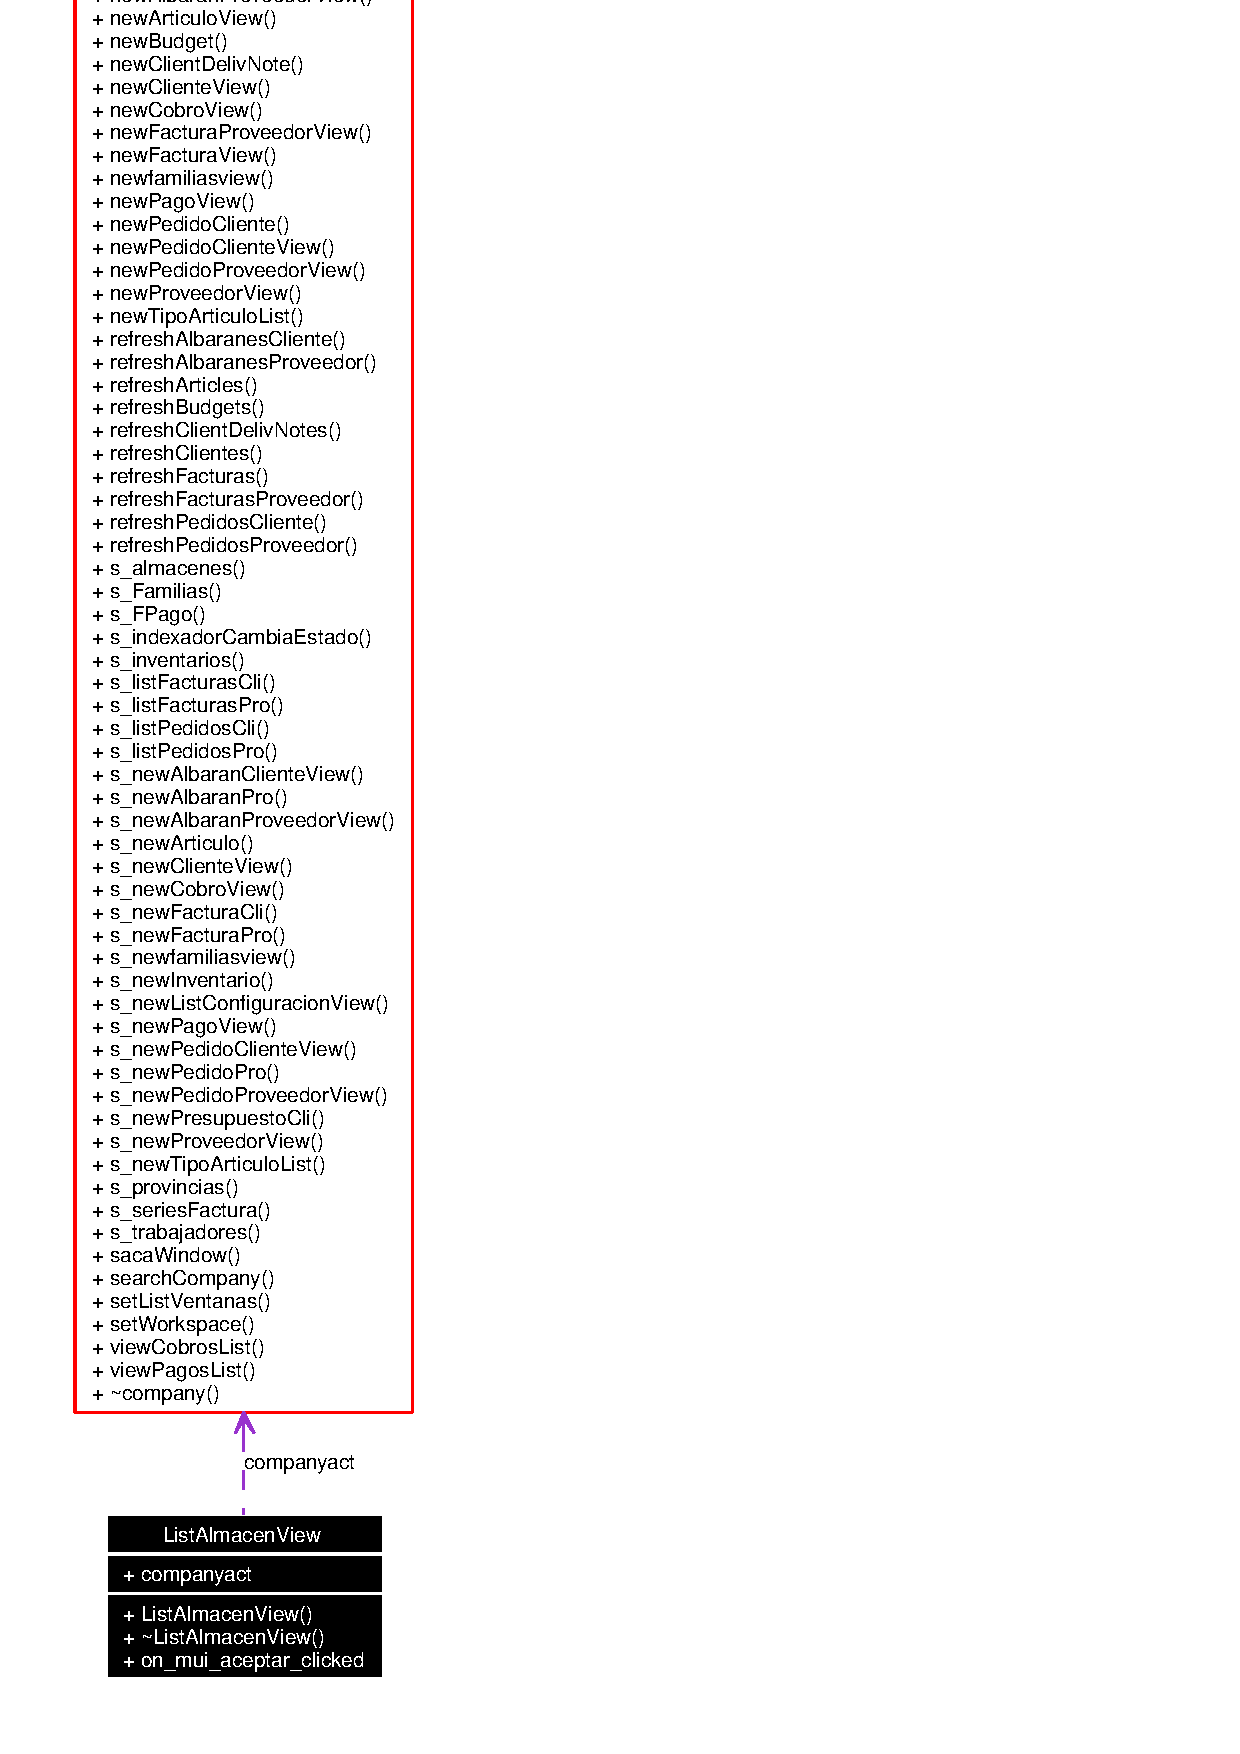
\includegraphics[width=99pt]{classListAlmacenView__coll__graph}
\end{center}
\end{figure}
\subsection*{Slots p\'{u}blicos}
\begin{CompactItemize}
\item 
virtual void {\bf on\_\-mui\_\-aceptar\_\-clicked} ()\label{classListAlmacenView_i0}

\end{CompactItemize}
\subsection*{M\'{e}todos p\'{u}blicos}
\begin{CompactItemize}
\item 
{\bf List\-Almacen\-View} ({\bf company} $\ast$comp, QWidget $\ast$parent)\label{classListAlmacenView_a0}

\end{CompactItemize}
\subsection*{Atributos p\'{u}blicos}
\begin{CompactItemize}
\item 
{\bf company} $\ast$ {\bf companyact}\label{classListAlmacenView_o0}

\end{CompactItemize}


\subsection{Descripci\'{o}n detallada}
Muestra y administra el listado de almacenes. 



La documentaci\'{o}n para esta clase fu\'{e} generada a partir de los siguientes archivos:\begin{CompactItemize}
\item 
listalmacenview.h\item 
listalmacenview.cpp\end{CompactItemize}
